Bisher wurde hauptsächlich der Energieverlust von Teilchen beim Durchqueren von Materie betrachtet,
nun werfen wir einen Blick auf die Änderung der Flugrichtung.
\\
Wir erinnern uns an den Rutherford-Wirkungsquerschnitt für die Streuung von geladenen Teilchen im
Coulomb-Feld eines Kerns:

\[ \frac{\mathrm{d}\sigma}{\mathrm{d}\Omega} = z^2Z^2\alpha^2\hbar^2 \frac{1}{\beta^2 p^2}\cdot
\frac{1}{4\text{sin}^4\cdot\frac{\Theta}{2}}
\]

\begin{figure}[H]
	\centering
	\includegraphics[width=0.5\textwidth]{rutherford.jpg}
	\caption{	 ???}
	\label{rutherford}
\end{figure}

Einfliegende Teilchen werden kohärent an der gesamten Ladung des Kerns gestreut ($\sim Z^2$???). Der
Energieverlust durch Ionisation ist proportional zu $Z$, da über Beiträge der Hüllenelektronen
inkohärent summiert wird.
\\ 
Ist $m_\text{gestreut} < m_\text{Kern}$, dann erfährt das Teilchen eine Richtungsänderung der
Flugrichtung bei geringem Energieübertrag. Man redet von Vielfachstreuung, wenn mehr als 20
Streuungen stattfinden (bei dickeren Schichten). Wir erhalten eine Gaußverteilung des Streuwinkelns
aufgrund des zentralen Grenzwertsatzes.

\begin{figure}[H]
	\centering
	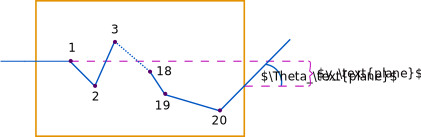
\includegraphics[width=0.5\textwidth]{vielfach.jpg}
	\caption{	 ???}
	\label{vielfach}
\end{figure}

Bei der Approximation durch eine Gaußverteilung wird die Streuwinkelverteilung durch einen
Parameter, der Standardabweichung $\Theta_0$ des in die Ebene projizierten Streuwinkels
$\Theta_\text{plane}$, festgelegt:

\[f(\Theta_\text{plane}) \mathrm{d}\Theta_\text{plane} =
\frac{1}{\sqrt{2\pi}\,\Theta_0} \,\text{exp}\left(-\frac{\Theta_\text{plane}^2}{2\Theta_0^2} \right)
\mathrm{d}\Theta_\text{plane}\]

Der Parameter $\Theta_0$ ist näherungsweise gegeben durch

\[\Theta_0 = \frac{13{,}6\,\text{MeV/c}}{p\cdot\beta} \cdot Z\cdot
\sqrt{\frac{x}{x_0}}\left(1+0{,}038\cdot\text{ln}\frac{x}{x_0} \right)   \]

mit dem Zusammenhang zum räumlichen Streuwinkel

\[\sqrt{\bar{\Theta}^2} = \sqrt{2}\cdot\Theta_0.  \]

Um durch den Detektor fliegende Teilchen zu simulieren, teilt man ihn in Streu-Schichten auf und
berechnet den Versatz und Streuwinkel am Austrittsort. Der mittlere Versatz ist

\[ \bar{y}_\text{plane} = \frac{1}{\sqrt{2}}\cdot x \cdot \Theta_0. \]

Diese Approximation ist innerhalb von $5\,$\% genau für Streudicken von $10^{-3}<\frac{x}{x_0}<10$
\begin{itemize}
  \item für Blei von etwa $5\,\mu$m bis $50\,$mm,
  \item für Luft von etwa $0{,}3\,$mm bis $3\,$m.
\end{itemize}


